\subsection{Datová vrstva IS}
Datová vrstva informačního systému \textbf{odděluje aplikaci od databáze}. Jde o třídy a funkce zajišťující komunikaci s databázi. \textbf{Překonává propast mezi SŘBD a programovacím jazykem}. Nazývá se také perzistentní a je 3. (nebo 1. záleží na úhlu pohledu) vrstvou \textbf{třívrstvé architektury} IS.

Jedná se třídy a funkce, které se starají o persistentní ukládání dat, odtud také název. Datová vrstva nemusí nutně ukládat data do databáze, ale klidně do JSONu, XML, nebo přes API na jiných serverech. Proto je oddělená, aby bylo možné měnit \uv{poskytovatele} dat. Proto se programátor nemusí starat o fyzické uložení dat, pouze o práci s nimi.

\begin{figure}[H]
	\centering
	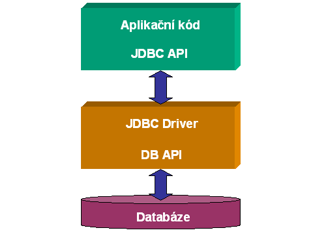
\includegraphics[width=0.48\textwidth]{assets/jdbc.png}
	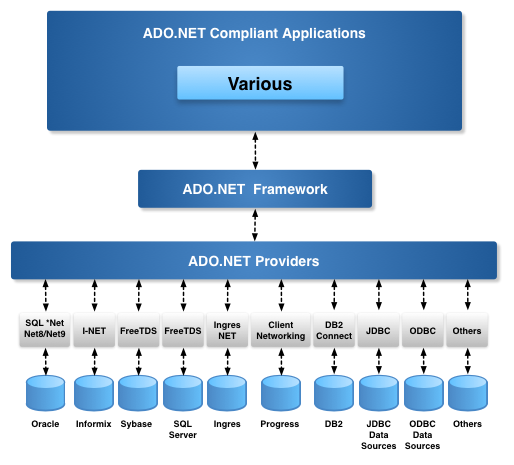
\includegraphics[width=0.4\textwidth]{assets/adonet.png}
\end{figure}

\begin{itemize}
\item \textbf{Nástroje} -- programovací jazyky + \textbf{SQL}, staví na \textbf{API pro dotazování DB} (JDBC, ADO.NET), \textbf{embedded SQL} - hostitelský jazyk obsahuje SQL.
\begin{itemize}
	\item \textbf{ODBC} (Open DataBase Conectivity) -- standartizované API pro přístup k databázovým systémům. ODBC se snaží poskytovat přístup nezávislý na programovacím jazyku, databazovem systému a operačním systému. 
	\item \textbf{JDBC} (Java DataBase Conectivity) -- Javovské API pro unifikovaný přístup k databazi. Bez ohledu kde jsou data uložena - SQL databáze, Oracle, XML, CSV, DB2, Ingress, ... -- se s nimi přes JDBC pracuje stejně.
	\item \textbf{ADO.NET} (Active Data Object) -- specifikace (knihovna) pro přísutupu k datový zdrojům na platformě .NET.
	\item \textbf{ASP.NET} -- knihovny pro informační systémy na platformě .NET. Pro komunikaci s databazi využívají ADO.NET.
	\item \textbf{Java2EE} -- knihovny pro informační systémy na platformě Java.
\end{itemize}
\item\textbf{Speciální prostředí} -- implementováno výrobcem SŘBD (Oracle Forms, APEX). Jednoduché, šité na míru, není připravené pro velké projekty a týmový vývoj.
\item \textbf{Architektury} -- jsou \textbf{komplikované}, \textbf{vícevrstvé}, ale umožňují jednodušší vývoj a zapojení více vývojářů. (3-vrstvá architektura => Business, Data, Presentation layer).
\end{itemize}

\subsubsection{JDBC}
\begin{itemize}
\item Rozhraní pro \textbf{unifikovaný přístup k datům} v DB na platformě \textbf{Java}.
\item Inspirováno rozhraním \textbf{ODBC}.
\item Zprostředkování komunikace aplikace s konkrétním typem DB (ovladače k většině).
\item \textbf{Dotazovací jazyk – SQL}. Předá se DB, ovladač vyhodnotí přímo.
\item \textbf{Schéma provedení dotazu:} 1) Připojení k datovému zdroji. 2) Inicializace. 3) Vytvoření a provedení dotazu. 4) Získání výsledku. 5) Ukončení transakce. 6) Odpojení od datového zdroje.
\item Hlavní třída \textbf{Connection} - odesílá \texttt{Statementy} a obdrží \texttt{ResultSety}.
\item \textbf{Podpora transakcí }(implicitně, každý příkaz jedna transakce, jsou vázány k instanci connection). 
\end{itemize}

\subsubsection{ADO.NET}
\begin{itemize}
\item \textbf{Connection} spouští \texttt{Commandy}, výsledkem je \texttt{DataSet} (použití \texttt{DataAdapteru}) nebo čistá data čtená \texttt{DataReaderem}.
\item \texttt{DataSet -> DataTable[] -> DataRow[] -> DataColumn[]}
\item \textbf{DataRelation} vazba mezi \texttt{DataSety} s vazebním \texttt{DataColumn}.
\item Umožňuje \textbf{parametrizovat commandy}.
\item Třída \textbf{\texttt{TransactionScope}} pro distribuované transakce.
\end{itemize}

\subsection{ORM (Objektově-relační mapování)}
Programovací technika \textbf{zpřístupňující relační či objektově-relační data pro objektové prostředí}. Entita v ORM je objekt, který je uložen v SŘBD (nejčastěji jako jeden záznam). Nejčastěji je implementován jako třída. Díky rozhraní jsou jednotlivé implementace zaměnitelné. Vlastnosti ORM rámců:
\begin{itemize} 
\item Práce s objektovým modelem (přenositelnost mezi různými SŘBD).
\item Překonává propast mezi SŘBD a programovacím jazykem.
\item \textbf{Rychlejší vytváření aplikací} vs Menší výkon aplikace.
\item Nemusí využívat všechny vlastnosti SŘBD (efektivita, bezpečnost apod.). Záleží na komplexnosti a kvalitě knihovny ORM.
\item Typová kontrola (nevznikají chyby v SQL).
\item Jednodušší testování.
\item Může využívate existující API jako JDBC, ADO.NET apod.
\item Měly by se používat pouze metody a parametry ORM, nikoli přímo SQL dotazy.
\item Využívá známé návrhové vzory \textbf{Table data gateway}, \textbf{Row data gateway}, \textbf{Active record}, \textbf{Data mapper}.
\item Dobré ORM si dokáže poradit i s dědičností pomocí návrhových vzorů \textbf{Single--table inheritance}, \textbf{Class table inheritance} a \textbf{Concrete table inheritance}.
\end{itemize}

\subsubsection{Pravidla ORM}
\begin{itemize}
\item \textbf{Minimalizace počtu dotazů }zasílaných na server.
\item \textbf{Minimalizovat objem dat} získaných z DB, stahovat pouze ta data, které potřebujeme, a které jsou zobrazeny uživateli (Lazy Loading).
\end{itemize}

\subsubsection{Vlastní implementace ORM}
\begin{itemize}
\item Využití \textbf{API pro komunikaci s DB} (JDBC, ADO.NET).
\item Používá se \textbf{SQL}.
\item \textbf{Výhody:} plná kontrola nad výkonem (stahujeme jen to co chceme) a prováděnými příkazy. Můžeme využít konkrétní prvky daného SŘBD.
\item \textbf{Nevýhody:} aplikace je závislá na určitém typu SŘBD, při rozšiřování systému je často nutné rozšířit také ORM.
\end{itemize}

\subsubsection{Automatizované}
\begin{itemize}
\item Frameworky \textbf{Hibernate} (Java), LINQ2SQL, \textbf{EntityFramework} (ASP.NET).
\item Může výrazně \textbf{degradovat výkon} (musí provádět interpretaci do SQL, vytváří objektový model atd.).
\item Většinou mají vlastní \textbf{cache}. Většinou jsou \textbf{nezávislé na daném SŘBD}.
\end{itemize}

\subsection{Bezpečnost}
\textbf{(Ne)Omezení práv} - uživatel může destruktivně vymazat celou DB, nebo číst data, která nemá. \textbf{Řešením} je omezení práv na jednotlivé akce, či úplné zamezení viditelnosti tabulek. Pro zobrazení jejich částí lze využít pohledy. 

\textbf{SQL Injection} - zranitelnost vznikající při nedostatečném \textbf{ošetření vstupů užívaných} v SQL dotazech. Např.: při přihlašování na webových stránkách zadá útoční příkaz SQL, které změní funkčnost dotazovaného příkazu. \textbf{Řešení:}
\begin{itemize}
\item \textbf{Parametrizované dotazy} (hodnoty jsou předány zvlášť, nemůže dojít k úpravě).
\item Uložené procedury.
\item Ošetření vstupů (\texttt{htmlspecialchars}, \texttt{mysql\_read\_escape\_string}) - zneužití např. pomocí jiného kódování!
\item Uživatel musí zadávat komplikovaná (neslovníková) hesla, \textbf{časové omezení počtu} pokusů. Logování neúspěšných pokusů o autentizaci.
\end{itemize}

\subsection{Způsoby doménově-relačního chování}
\begin{itemize}
    \item \textbf{Table data gateway} - Vrací Dataset DTO bez znalosti domény. Dataset obsahuje pole řádků, i když je navrácen pouze 1. Jediná instance drží i více řádků tabulky. Protože nezná doménu, každá funkce obsahuje tolik parametrů, kolik je sloupců. 
    \item \textbf{Row data gateway} - Každý řádek je 1 objekt. Obsahuje funkce pro \texttt{update} \texttt{delete}. Je potřebná nějaká statická třída \texttt{Finder} pro vytváření nových instancí, protože pokud nejsou data, neexistuje ani objekt.
    \item \textbf{Active record} - Každá instance je 1 řádek. Obsahuje i funkce \texttt{insert} a \texttt{update} atd. Ale také metody pro práci v programu, různé výpočetní apod.
    \item \textbf{Data mapper} - Mapper třída mapuje z DB data na objekty a zpět. Každý objekt obsahuje veškeré parametry a také funkce pro práci s nimi na úrovni programu. Do mapperu se nevkládají jednotlivá data jako parametry ale vždy daný objekt, který samotný funkce pro práci s DB postrádá.
\end{itemize}
